\setcounter{page}{1} 
\section{A Prelude to Pulsars}
When stars with a mass of at least $8 \smass$ reach the end of their evolutionary stage and experience a depletion of nuclear fuel will undergo a core collapse and explode as a Supernovae. Depending on the mass of the host star the Supernova will form a Black Hole or a Neutron Star. Based on the electron degeneracy pressure limit (Chan 1967) stars that fall in the range of 20 - 30 $\smass$ form neutron stars (need citation). \\

Neutron stars are supported against further collapse by the presence of neutron degeneracy pressure which arises from the Pauli exclusion principle. Strong Nuclear forces between the neutrons also provides additional support against gravatational collapse. With these two opposing forces a stable equilibrium is formed. \\ 

In turn, this makes neutron stars exceptionally dense, they become the densest known objects in the universe that emit light. The average density of a neutron star is $10^{17} \text{kg/m}^3$ (need citation). The radius of neutron stars are comparable to the size of cities, with radii of 10 - 20 km. \\

During collapse the conservation of magnetic flux plays a crucial role in the large strength magnetic fields that are observed in neutron stars along with contributions from the dynamo effect and frozen-in magnetic fields. The magnetic field of a neutron star are of the order of $10^{12}$ - $10^{15}$ Gauss (Need citation). \\

Charged particles accelerate along the magnetic field lines in the magnetosphere of the neutron star. The particles emit electromagnetic radiation in a cone shape along the magnetic axis. If the magnetic axis is not aligned with the rotational axis of the neutron star, the radiation beam will sweep across the sky. This is known as a pulsar and are analogus to cosmic lighthouses.  \\

\subsection{The Population of Pulsars}

As of writing there are currently more than 3380 known pulsars. Since their discovery in 1967 by Jocelyn Bell Burnell the population has grown immensly but there remains many questions about pulsar evolution and the subclasses that lie within the population as a whole. Similarly to how exoplanet popilations are shown using the mass-radius diagram and stellar populations are shown using the Hertzsprung-Russell diagram, pulsar populations are shown using what is known as the $P-\dot P$ diagram. \\

$P$ representing the Pulsar's rotational period and $\dot P$ it's derivative. These are key ways that pulsars are classified and study in context of their evolution. An example of a $P-\dot P$ diagram is shown in \cref{fig:p-pdot}. Different values on the plot indicate the roughly the Pulsars age and magnetic field strength. \Cref{fig:p-pdot} shows the vastly different values bettween pulsars in the milisecond range and pulsars in the second range. \\ 

Theoretically it has been shown that pulsars exhibit a death line in the $P-\dot P$ diagram. This is the line where pulsars are no longer able to emit radio waves. This is due to the fact that the pulsar's magnetic field is no longer strong enough to accelerate particles along the magnetic field lines. However it has been shown that pulsars do exist below this line. The area below this line is commonly referred to as the "graveyard". \\
\begin{figure}
    \centering
    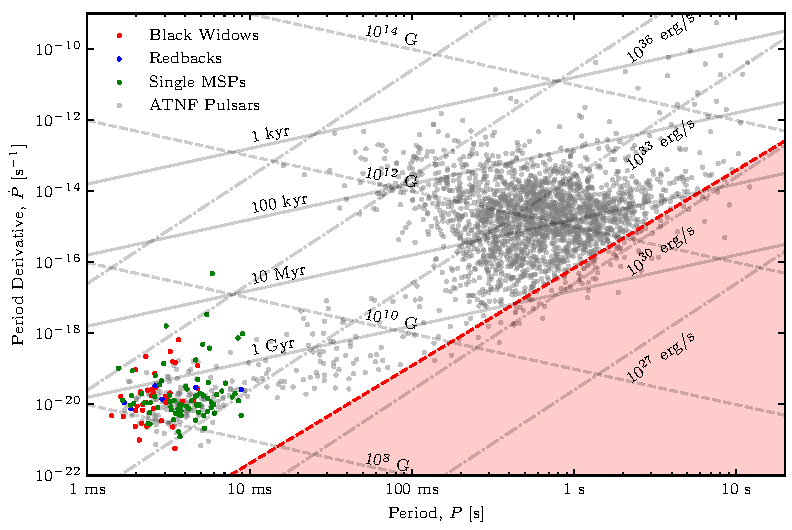
\includegraphics[width=0.8\textwidth]{figs/PPdot-diagram.pdf}
    \caption{The $P-\dot P$ diagram showing the population of pulsars. The pulsars are colour coded based on subclass. (cite ATNF)}
    \label{fig:p-pdot}
\end{figure}

\subsection{Pulsar Subclasses}

The population of pulsars can be broken down into subclasses based on unique patterns in their properities. The main subclasses\footnote{This is a non-exhaustive list.} are as follows:

\begin{enumerate}
    \item Normal Pulsars: These are the most common type of pulsars. They are characterized by their regular pulses and are often observed in radio wavelengths. They are also known as radio pulsars. %they cover central region of the $P-\dot P$ diagram.

    \item Rotating Radio Transients (RRATs): These are a subclass of pulsars that were initially discovered through their sporadic radio bursts rather than regular pulses. They exhibit irregular and infrequent radio emission.

    \item Magnetars: While not exclusively pulsars, magnetars are highly-magnetized neutron stars that can also emit pulsed radiation. They are characterized by extremely strong magnetic fields, much more intense than typical pulsars.

    \item Binary Pulsars: These are pulsars that are in orbit around another star, usually a normal (non-neutron) star. The interaction with the companion star can have significant effects on the pulsar's behavior, and studying binary pulsars has provided important tests of theories of gravitation.

    \item Millisecond Pulsars (MSPs): These are pulsars with very short rotation periods, typically less than 10 milliseconds. They are believed to be old pulsars that have been spun up by the accretion of mass from a companion star in a binary system.

    \item Gamma-ray Pulsars: Pulsars that emit pulsed gamma-ray radiation are known as gamma-ray pulsars. These are often detected by space-based telescopes like the Fermi Gamma-ray Space Telescope.

    \item X-ray Pulsars: Pulsars that emit pulsed X-ray radiation fall into this category. These pulsars are typically observed in binary systems where the pulsar accretes matter from its companion star, leading to X-ray emission.

    \item Anomalous X-ray Pulsars (AXPs) and Soft Gamma-ray Repeaters (SGRs): These are closely related to magnetars and are characterized by their intense and variable X-ray and gamma-ray emission. They are believed to be neutron stars with extremely strong magnetic fields.
\end{enumerate}

\subsection{Spider Pulsars}

The type of pulsar that is of interest to this project is a subclass of transional miliscond pulsars known as Spider Pulsars. Spider pulsars fall into two categories depending on their orbiting companion. The first category are known as Black Widow pulsars segreated based on their companion mass falling in the range of 0.01 - 0.05 $\smass$ with a compantion orbital period ($P_B$) of less than 10 hours (citation). The second category are known as Redback pulsars and have a companion mass of 0.2 $\smass$ or greater with a $P_B$ of less than 1 day (citation). \\ 


\subsubsection{4FGL J0523-2529}

\subsubsection{4FGL J2054-6904}